\documentclass[titlepage, 12pt]{article}
\usepackage[utf8]{inputenc}
\usepackage{multirow}
\usepackage{graphicx}
\usepackage[english,serbian]{babel}

\title{Luis fon An\\ \small{Seminarski rad u okviru kursa\\Tehničko i naučno pisanje\\ Matematički fakultet}}
\author{Aleksandar Šmigić \\ mi19028@alas.matf.bg.ac.rs \and Andrijana Milić \\ mi18186@alas.matf.bg.ac.rs \and Miloš Petričković \\ mi18055@alas.matf.bg.ac.rs \and Nikola Milutinović \\ mi18202@alas.matf.bg.ac.rs}
\date{Novembar 2019}

\begin{document}

\maketitle

\tableofcontents
\newpage
\section{Uvod}

{\renewcommand{\arraystretch}{1.2}}
\begin{tabular}{|c|c|c|}
\hline
\multicolumn{2}{|c|}{\Large{Luis fon An}}\\[4px]
\hline
\multicolumn{2}{|c|}{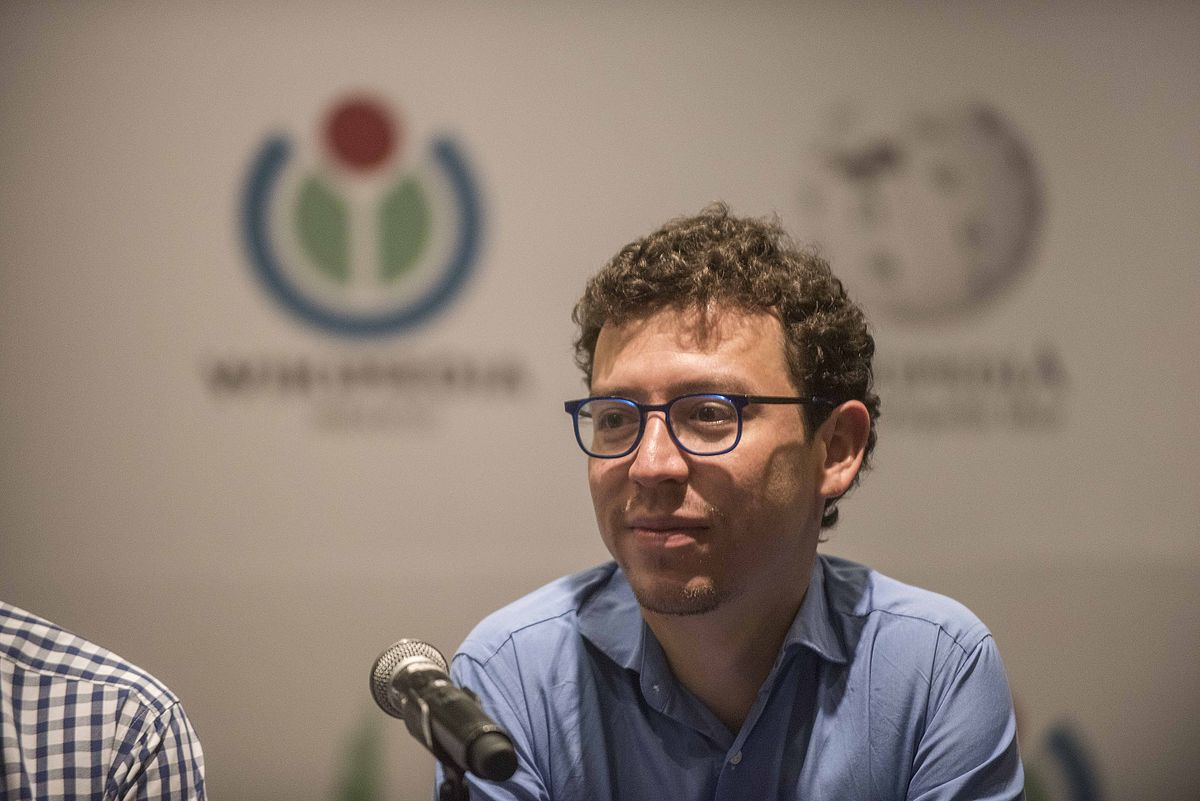
\includegraphics[width=320px,height=216px]{Luis_von_Ahn.jpg}}\\

\hline
Datum rođenja & 19.8.1955. \\
\hline
Mesto rođenja & Gvatemala, Gvatemala\\
\hline
Prebivalište & Berkli(Kalifornija)\\
\hline
\multirow{2}{*}{Institucije}&Univerzitet Karnegi Melon\\
& Univerzitet Djuk \\
\hline 
\multirow{3}{*}{Poznat po} & CAPTCHA \\
& reCAPTCHA \\ & Duolingo \\
\hline
\multirow{2}{*}{Nagrade} & MacArthur Fellowship (2006) \\
 & TR35 (2007)
\\
\hline
\end{tabular}

\vspace{20px}

Luis fon An, rođen 19. avgusta 1978. je gvatemalski preduzetnik i profesor konsultant na odseku za računarstvo na univerzitetu Karnegi Melon u Pitsburgu u Pensilvaniji.[1] Poznat je kao jedan od začetnika crowdsourcing-a. On je osnivač kompanije reKapča (engl. reCAPTCHA), koja je prodata Guglu 2009. godine, [2] i jedan od osnivača i glavni izvršni direktor Duolinga, popularne platforme za učenje jezika. 

\section{Biografija}
Fon An je rođen i odrastao u Gvatemali. On je nemačko-gvatemalskog porekla. 
Osnovne studije iz matematike (\textit{summa cum laude}) je završio na Djuk univerzitetu 2000. godine, a kasnije doktorat iz računarstva na Karnegi Melon univerzitetu 2005.
Fon An je 2006. godine postao fakultetski član Karnegi Melon škole računarstva na univerzitetu Karnegi Melon.

\section{Rad}
Kao profesor, njegova istraživanja uključuju \textit{CAPTCHA} i \textit{human computation}, čime je stekao svoju svetsku prepoznatljivost i brojne nagrade. Nagrađen je \textit{MacArthur Fellowship 2006}, \textit{David and Lucile Packard Foundation Fellowship 2009, Sloan Fellowship 2009, Microsoft New Faculty Fellowship 2007. i Presidental Early Career Award for Scientists and Engineers 2012}. Takođe je bio imenovan jednim od 50 najvećih umova u nauci od strane \textit{Discover}, i dospeo je do mnogih uglednih listi kao što su \textit{Briliant 10} od \textit{Popular Science}, \textit{50 Most Influential People in Technology} od \textit{Silicon.com}, \textit{TR35: Young Innovators Under 35} od \textit{MIT Technology Review i 100 Most Innovative People in Business} od \textit{Fast Company}. 
\textit{Siglo Veintiuno}, jedna od najvećih novina u Gvatemali, izabrala ga je za osobu godine 2009. \textit{Foreign Policy Magazine} na španskom ga je 2011. imenovao za najuticajnijeg intelektualca Latinske Amerike i Španije. 
Fon An je svoja istraživanja započeo na polju kriptografije. Zajedno sa Nikolasom Huperom i Džonom Langfordom, prvi je obezbedio precizne definicije steganografije i dokazao da je steganografija sa ličnim ključem moguća.

Godine 2000, u saradnji sa Manuelom Blumom, bavio se pionirskim radom na \textit{CAPTCHA} sistemu - kompjuterski generisanim testovima koje ljudi mogu jednostavno da urade, ali koje računari nisu u stanju da reše. Ovaj sistem koriste internet stranice da bi sprečile automatizovane programe, botove, da počine zloupotrebu velikih razmera, kao što je automatsko registrovanje mnogobrojnih naloga ili kupovina velikog broja ulaznica koje bi preprodavci kasnije preprodavali. \textit{CAPTCHA} je proslavila Fon Ana pred širokim auditorijumom zbog toga što su o njoj članke objavili \textit{New York Times} i \textit{USA Today} i što je propraćena na kanalima \textit{Discovery Channel}, \textit{NOVA scienceNOW} i ostalim popularnim medijima.

Fon Anova doktorska teza, završena 2005. godine, bio je prvi stručni rad koji je koristio termin \textbf{/human computation/}, koga je smislio Fon An sa željom da opiše metode koje kombinuju ljudsku inteligenciju i računare da bi rešile probleme koji u suprotnom ne bi mogli da se reše. Fon Anova doktorska teza je takođe prvi stručni rad na temu \textbf{/Igre sa poentom/} (\textit{Games With A Purpose - GWAP}). Igre sa poentom su igre koje, kao propratni efekat, izvode korisne proračune. Najpoznatiji primer je \textit{ESP Game}, onlajn igra tokom koje se nasumičnom paru igraca bez mogućnosti komunikacije istovremeno prikazuje ista slika koju oni treba da opišu u ograničenom vremenu, za šta dobijaju poene. Na osnovu ove igre dobija se precizan opis slike koji može biti uspešno upotrebljen u bazi podataka za poboljšavanje tehnologije pretrage slika. Gugl je licencirao \textit{ESP Game} u obliku Gugl obeleživača slika (engl. \textit{Google Image Labeler}) i koristi se da poboljša preciznost Gugl pretraživača slika (engl. \textit{Google Image Search}). Fon Anova igra donela mu je pažnju popularnih medija. Njegova teza osvojila je nagradu najbolje doktorske disertacije škole računarskih nauka univerziteta Karnegi Melon. Jula 2006, Fon An je održao govor u Guglu o \textit{/Human Computation/} (tj. \textit{crowdsourcing}) koji je imao preko milion gledalaca.


Fon An je 2007. godine izumeo \textit{reCAPTCHA}, novi oblik \textit{CAPTCHA} koji takode pomaže pri digitalizaciji knjiga. Slike reči koje koristi \textit{reCAPTCHA} dolaze direktno iz starih knjiga nakon što su digitalizovane; koriste se reči koje optičko prepoznavanje znakova ne bi moglo da prepozna i šalju se ljudima putem mreže kako bi se identifikovali. \textit{reCAPTCHA} se trenutno koristi na preko 100.000 veb-sajtova i prevodi preko 40 miliona reči dnevno.

Godine 2011. dodeljena mu je nagrada A. Niko Habermana, predsedavajućeg za razvoj u računarskim naukama, koja se dodeljuje svake treće godine obećavajućem mladom članu fakulteta u školi računarskih nauka.

Fon An 2018. godine osvojio je \textit{Lemelson-MIT} nagradu za /njegovu posvećenost poboljšanju sveta kroz tehnologiju/.

Od 2014. Fon An je generalni direktor Duolinga, platforme za učenje jezika.


\section{Učenje}

Fon An je koristio mnoge neobične tehnike u svojoj nastavi koje su mu donele brojne nagrade Univerziteta u Karnegi Melonu. Jeseni 2008. godine započeo je novi kurs na Karnegi Melonu sa nazivom „Nauka mreža” (engl. Science of the Web). Kombinacija teorije grafova i društvenih nauka, kurs obrađuje teme od teorije mreža i teorije igara do teorija aukcije.

\begin{thebibliography}{9}
\bibitem{ref1}
    \textit{„Luis von Ahn”.}
\bibitem{ref2}
    \textit{„Teaching computers to read: Google acquires reCAPTCHA”. Google Official Blog.}
\bibitem{ref3}
    \textit{„Duke Ugrad Alum Profile: Luis von Ahn”.}
\bibitem{ref4}
    \textit{https://www.cs.cmu.edu/~biglou/LuisvonAhnCV.pdf}
\bibitem{ref5}
    \textit{Federoff, Stacey. „Duolingo CEO Luis von Ahn wins Lemelson prize from MIT”.}
\bibitem{ref6} 
    \textit{Robert J. Simmons. „Profile Luis von Ahn: ReCaptcha, games with a purpose”. XRDS: Crossroads, the ACM Magazine for Students.}
\bibitem{ref7}
    \textit{„MacArthur Fellows”.}
\bibitem{ref8}
    \textit{„Congratulations, Luis von Ahn”. Google Official Blog.}
\bibitem{ref9}
    \textit{„President Obama Honors Outstanding Early-Career Scientists”. The White House.}
\bibitem{ref10}
    \textit{„Los nuevos rostros del pensiamento iberoamericano”. FP.}
\bibitem{ref11} 
    \textit{„Luis von Ahn”.}
\bibitem{ref12} 
    \textit{Von Ahn, Luis; Blum, Manuel; Hopper, Nicholas J.; Langford, John). "CAPTCHA: Using Hard AI Problems for Security". Proceedings of the International Conference on the Theory and Applications of Cryptographic Techniques}
\bibitem{ref13}
    \textit{Von Ahn, L.; Blum, M.; Langford, J. „Telling humans and computers apart automatically”. Communications of the ACM.}
\bibitem{ref14}
    \textit{Von Ahn, L.; Dabbish, L. „Labeling images with a computer game”. Proceedings of the conference on Human factors in computing systems}
\bibitem{ref15}
    \textit{Von Ahn, L. „Games with a Purpose”.}
\bibitem{ref16} Google Tech Talk on human computation by Luis von Ahn.
\bibitem{ref17}
    \textit{„reCAPTCHA (a.k.a. Those Infernal Squiggly Words) Almost Done Digitizing the New York Times Archive”. Blog.newsweek.com.}
\bibitem{ref18}
    \textit{Habermmann Chair announcement. News.cs.cmu.edu}
\bibitem{ref19}
    \textit{Federoff, Stacey. „Duolingo CEO Luis von Ahn wins Lemelson prize from MIT”. TribLIVE.com.}
\bibitem{ref20}
    \textit{Duolingo.com}
\bibitem{ref21}
    \textit{CMU Faculty Awards.}
\bibitem{ref22}
    \textit{„Science of the Web”. Andrew.cmu.edu.}
\end{thebibliography}

\end{document}
